In \autoref{fig:eval_vanilla}, the evaluation of the interaction introduced above is shown for the three training nuclei.

% Varbound
An important metric in assessing our extrapolation comes from the variational principles of NCSM calculations for ground-state energies. Since the energies decrease mononously with increasing model-space dimensions, it is guarantied that the exact ground-state energy is lower than all computed NCSM values, regardless of model-space dimension. As a consequence, we can require from a reasonable extrapolation, that the extrapolated energy is lower than the lowest value at the maximum $N_\mathrm{max}$. This mimimum value is called the \textit{variational boundary}. For all maximum $N_\mathrm{max}$ in \autoref{fig:eval_vanilla}, those variational boundaries are shown as dashed lines. We can see that this condition is fulfilled for all nuclei in the case of a flow parameter of \srg{0.04}. This condition only fails for the extrapolations of \n{2}{H} with a flow parameter of \srg{0.08}. Additionally, we can also compare the extrapolation result to the variational boundary of the highest $N_\mathrm{max}$ available, as this provides a further upper bound for the exact ground-state energy. This upper bound is also interesting because it is not directly nor indirectly input into the networks, in contrast to the variational boundaries at the maximum $N_\mathrm{max}$, and thus represents a stronger condition for the extrapolation quality of the networks. For the nuclei \n{3}{H} and \n{4}{H}, this condition is also fulfilled. The extrapolations of the energies for the \n{2}{H} nucleus consistently fail to meet this condition.

\begin{figure}[H]
  \centering
  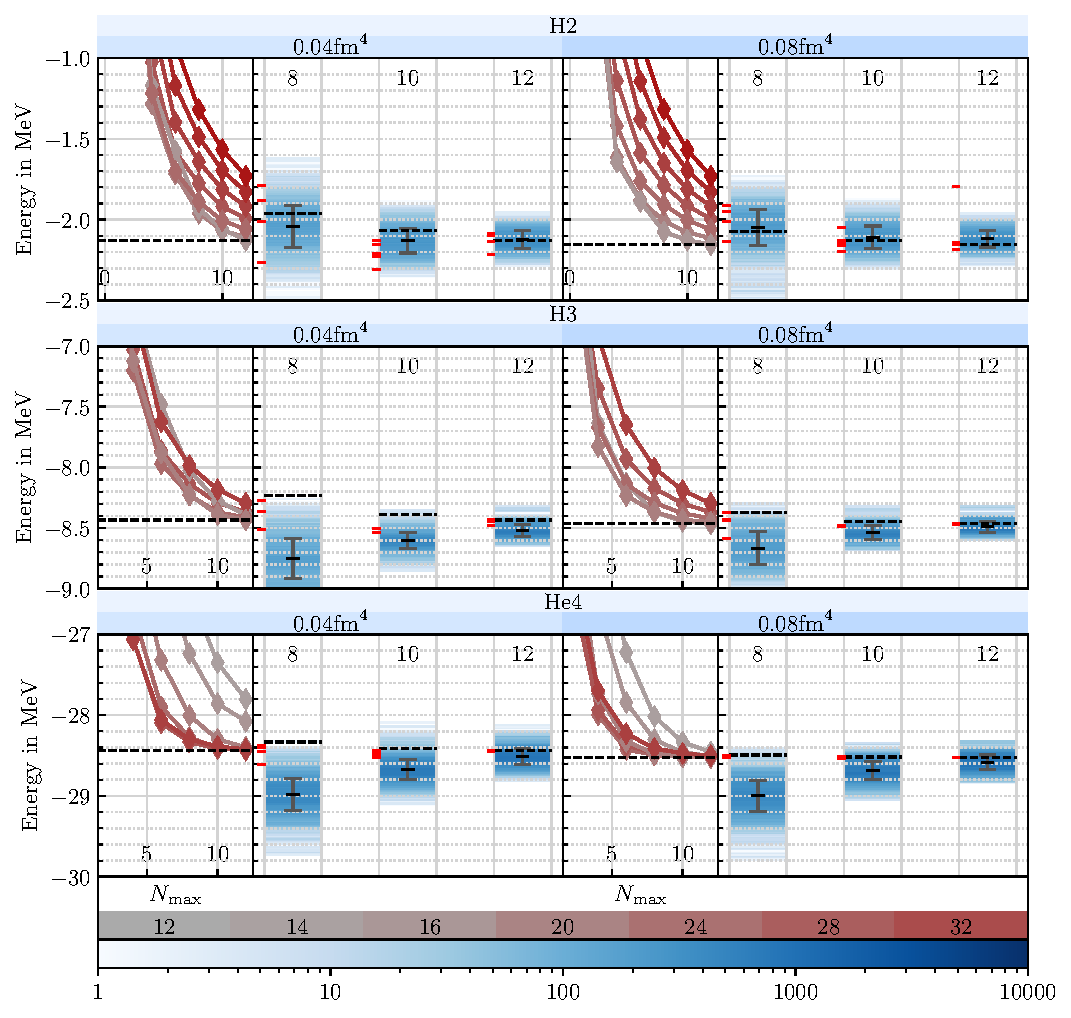
\includegraphics[width=\textwidth]{media/vanilla_evaluation.pdf}
  \caption{Evaluation of our extrapolation method on the nuclei \n{2}{H}, \n{3}{H} and \n{4}{He}, using a semi-local momentum space regulated $N^{2}LO$ interaction with two-body interactions and a cutoff at \SI{450}{\mega\electronvolt}. For each nucleus and each flow parameter, the NCSM sequences are shown on the left (the different frequencies are colored respectively to the legend, which shows the frequencies $\hbar\Omega$ in \si[]{\mega\electronvolt}) and the extrapolations for a given maximum $N_\mathrm{max}$ on the right. For each maximum $N_\mathrm{max}$, the variational boundary is shown as a dashed line, and the classical extrapolations are shown as red ticks.}
  \label{fig:eval_vanilla}
\end{figure}

% Better with higher Nmax
On first sight, the network predictions get more precise when we restrict the evaluation samples to higher values of $N_\mathrm{max}$. This indicates that the networks associate steeper slopes of energy sequences with sequences that are not converged already as well as flat sequences with sequences that are more converged. Based on this, the network tries to extrapolate the steeper sequences with lower predictions and flatter sequences with higher predictions, that lie more closely to the variational boundary. In fact, for the lower values of $N_\mathrm{max}$, the networks generally predict a value for the ground-state energy which is too low in comparison to the variational boundary at the given $N_\mathrm{max}$ or even the variational boundary for the highest available $N_\mathrm{max}$, which is drawn as a dashed line on the left side of the plots.

Additionally, since the sequences for the different oscillator frequencies converge at different rates, they are further apart for lower $N_\mathrm{max}$ and thus the network extrapolates them on a broader range of energies, resulting in a bigger uncertainties for smaller $N_\mathrm{max}$.

% H2 vs rest -> slowest to converge?
An exception to this general extrapolation behaviour of extrapolating unreasonably low values for smaller $N_\mathrm{max}$ and correcting the predictions towards the variational boundary for higher $N_\mathrm{max}$ is the nucleus \n{2}{H}. Here, our network shows a systematically different extrapolation behaviour. First, the networks extrapolate the energies not far enough for all $N_\mathrm{max}$. Secondly, the predictions generally get lower if the maximum $N_\mathrm{max}$ of the evaluation samples is increased. This may originate from the fact that the NCSM calculations for \n{2}{H} are the slowest to converge among the three nuclei. The slow convergence results in some sequences having a much flatter slope while still being too high in value with respect to the variational boundary, which is determined by the fastest converging sequence. Another possible origin of this systematic difference is that the training set of nuclei is not balanced evenly between the nuclei and \n{2}{H} may be underrepresented, such that the slow convergence behaviour of \n{2}{H} is foreign to the networks.

% 0.04 vs 0.08
If we look at the differences between the two SRG flow parameters of \srg{0.04} and \srg{0.08}, we cannot find a systematic differences but a general shift of the extrapolations to higher values with respect to their variational boundaries. This is not surprising, since a higher SRG flow parameter leads to faster convergence of the NCSM sequences. It results in lower variational boundaries as well as in a higher extrapolation, which is an effect we already observed in the \n{2}{H} extrapolations.
